% !TeX spellcheck = ru_RU
% !TEX root = vkr.tex

\section{Особенности реализации программного инструмента для определения профориентационных предпочтений}

В разделе приведены технические детали реализации проекта: используемые языки и библиотеки, описание набора данных, архитектура кода и ключевые функции для подготовки данных, построения и оценки моделей (регрессия, классификация, ранжирование, ансамблирование), а также структура прототипа веб-приложения на R Shiny.


\subsection{Общие особенности реализации}

Реализация моделей определения профориентационных предпочтений на основе психометрических тестов личности производилась на языке R (версия 4.4.2)\footnote{\quad R Core Team. \textit{R: A Language and Environment for Statistical Computing}. R Foundation for Statistical Computing, Vienna, Austria.~--- 2024. URL: \url{https://www.R-project.org/} (дата обращения: 17.05.2025).}, являющимся открытым и свободным программным обеспечением. Язык R обеспечивает эффективность обработки данных за счёт векторизованных операций и оптимизированных реализаций статистических алгоритмов в базовых и дополнительных пакетах. Для обработки данных преимущественно использовались библиотеки \emph{data.table} для эффективных табличных преобразований, \emph{tidyverse} (различные манипуляции с данными \emph{dplyr}, элементы функционального программирования с \emph{purrr}, работа со строками через \emph{stringr}), \emph{arrow} для передачи наборов данных между R и Python, визуализация в \emph{plotly}. Нейросетевые модели реализованы на языке Python (версия 3.12.3)\footnote{\quad Van Rossum G, Drake FL. Python 3 Reference Manual. Scotts Valley, CA: CreateSpace.~--- 2009.} с использованием открытого и свободного ПО: \emph{numpy} и \emph{pandas} для численных вычислений и подготовки данных, \emph{PyTorch} как гибкий фреймворк для построения и обучения глубоких нейронных сетей.

Исходный код всего проекта представлен в GitHub-репозитории\footnote{\quad GitHub: Предсказание кода Голланда (RIASEC) по результатам психометрических тестов личности. URL: \url{https://github.com/ExP98/Diploma_Holland} (дата обращения: 17.05.2025).}. В репозитории представлена программная реализация вычислительного эксперимента, представленного на рисунке~\ref{fig:multi_pipeline}. Далее будут описаны ключевые шаги эксперимента с упоминанием названий функций и используемых библиотек, однако описание кода не является исчерпывающим. Код на языке R написан в соответствии с руководством по стилю оформления кода \emph{Tidyverse Style Guide}\footnote{\quad Руководство по стилю оформления кода на языке R. Tidyverse Style Guide. URL: \url{https://style.tidyverse.org/} (дата обращения: 17.05.2025).}, что обеспечивает единообразие оформления, читаемость и простоту сопровождения.

Инструмент автоматизации процесса профориентации состоит из следующих модулей:
\begin{itemize}
    \item модуль обработки данных;
    \item модуль восстановления данных;
    \item модуль обучения базовых моделей;
    \item модуль формирования взвешенного ансамбля моделей;
    \item модуль организации и проведения вычислительных экспериментов.
\end{itemize}
Предварительно проводился разведочный анализ данных. По результатам вычислительного эксперимента происходил выбор наилучших подходов для определения кода Голланда, обучение и сохранение лучшей модели. На её основе реализуется прототип инструмента автоматизации профориентации: веб-приложение на основе R Shiny.


\subsection{Описание набора данных. Разведочный анализ}

Данные для исследования были собраны с помощью опросов, размещенных в веб-приложении на базе платформы VK Mini Apps \enquote{Психологические тесты}\footnote{\quad Мини-приложение \enquote{Психологические тесты} (платформа \enquote{VK Mini Apps}). URL: \url{https://vk.com/app7794698} (дата обращения: 17.05.2025).}~\cite{vk_psychotests}. Приложение находится в открытом доступе и позволяет пользователям проходить различные психометрические опросы, при этом после ознакомления с условиями добровольного информированного согласия\footnote{\quad Политика конфиденциальности. URL: \url{https://vk.com/@ticslabs-politika-konfidencialnosti} (дата обращения: 17.05.2025).} пользователи могут разрешить использовать обезличенные анонимизированные данные в научных исследованиях (в соответствии с №~152-ФЗ \enquote{О персональных данных}).

\begin{figure}[bhtp]
    \centering
    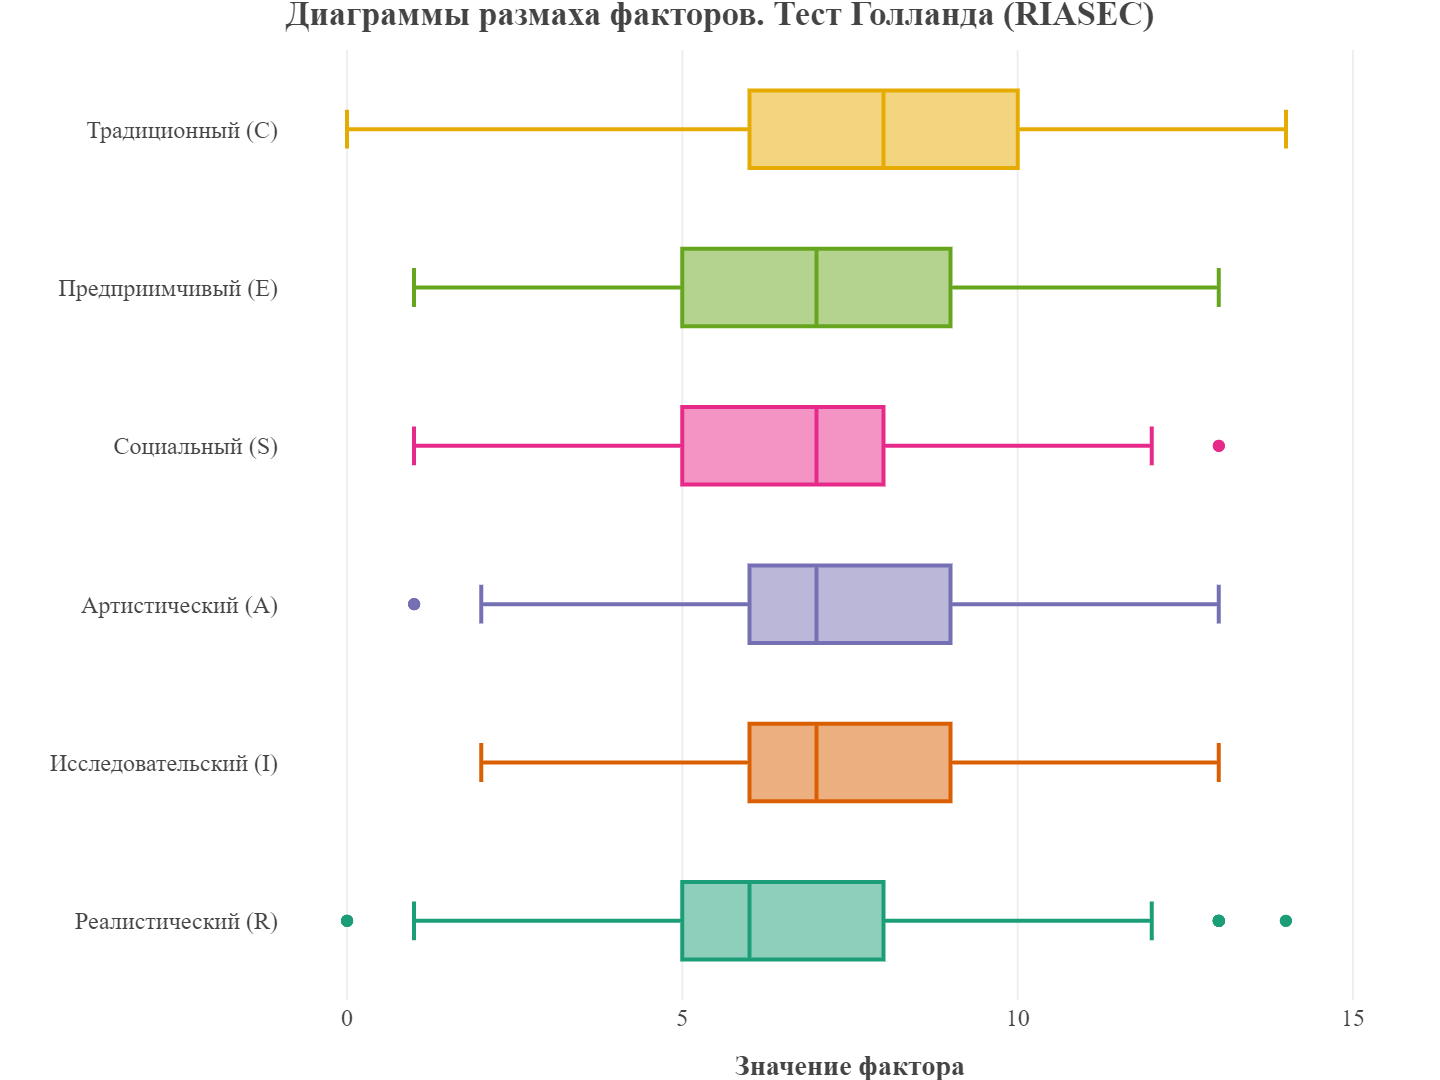
\includegraphics[width=0.75\linewidth]{figures/HL.png}
    \caption{Диаграмма размаха факторов модели Голланда}
    \label{fig:HL_boxplot}
\end{figure}

В наборе представлены данные по следующим психометрическим тестам (в скобках указано количество факторов):
\begin{enumerate}[noitemsep, topsep=4pt]
    \item Опросник Леонгарда-Шмишека (10).
    \item Личностный опросник Айзенка (4).
    \item 16-факторный опросник Кеттелла (16).
    \item Пятифакторный опросник личности (\enquote{Большая пятёрка}; 5).
    \item Ценностный опросник Шварца (20).
\end{enumerate}
Более подробное описание тестов и их факторов представлено в подразделе~\ref{sec:psytests}. Всего имеются данные по 1278 пользователям: у 339 есть данные по всем тестам, у 939 пользователей отсутствует один или два теста. Пример части преобразованного набора данных представлен в таблице~\ref{tab:input_test_data}. Диаграмма размаха для факторов модели Голланда представлена на рисунке~\ref{fig:HL_boxplot}, плотность их фактических значений~--- на рисунке~\ref{fig:facet}, частоты значений кодов в порядке убывания их значимости~--- рисунок~\ref{fig:ranks}. 

\begin{figure}[bhtp]
    \centering
    \begin{minipage}[b]{0.49\linewidth}
        \centering
        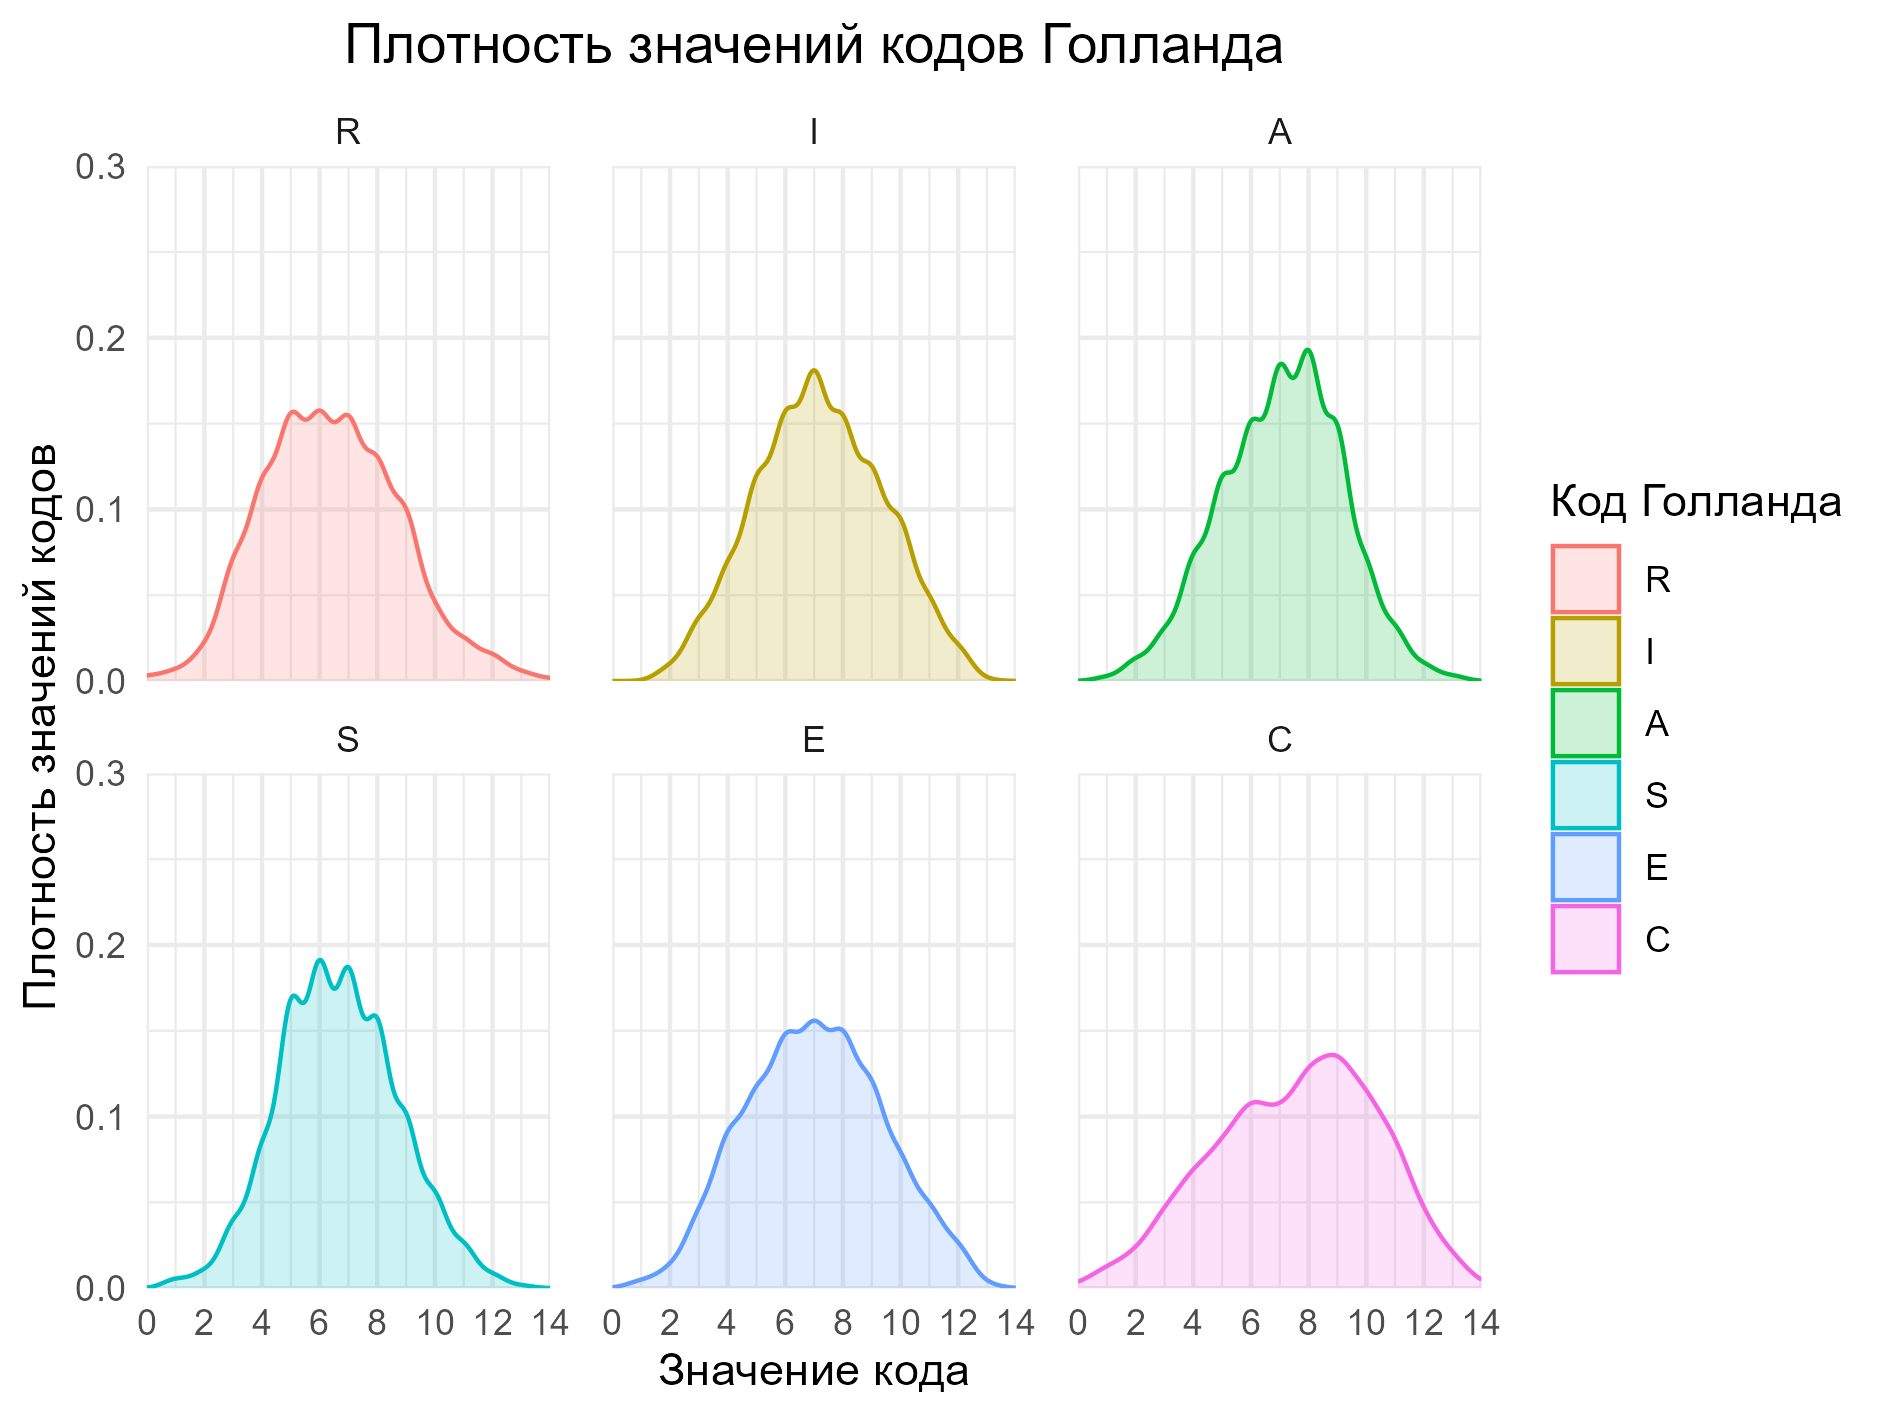
\includegraphics[width=\linewidth]{figures/facet.png}
        \caption{Плотность фактических значений кодов Голланда}
        \label{fig:facet}
    \end{minipage}
    \hfill
    \begin{minipage}[b]{0.49\linewidth}
        \centering
        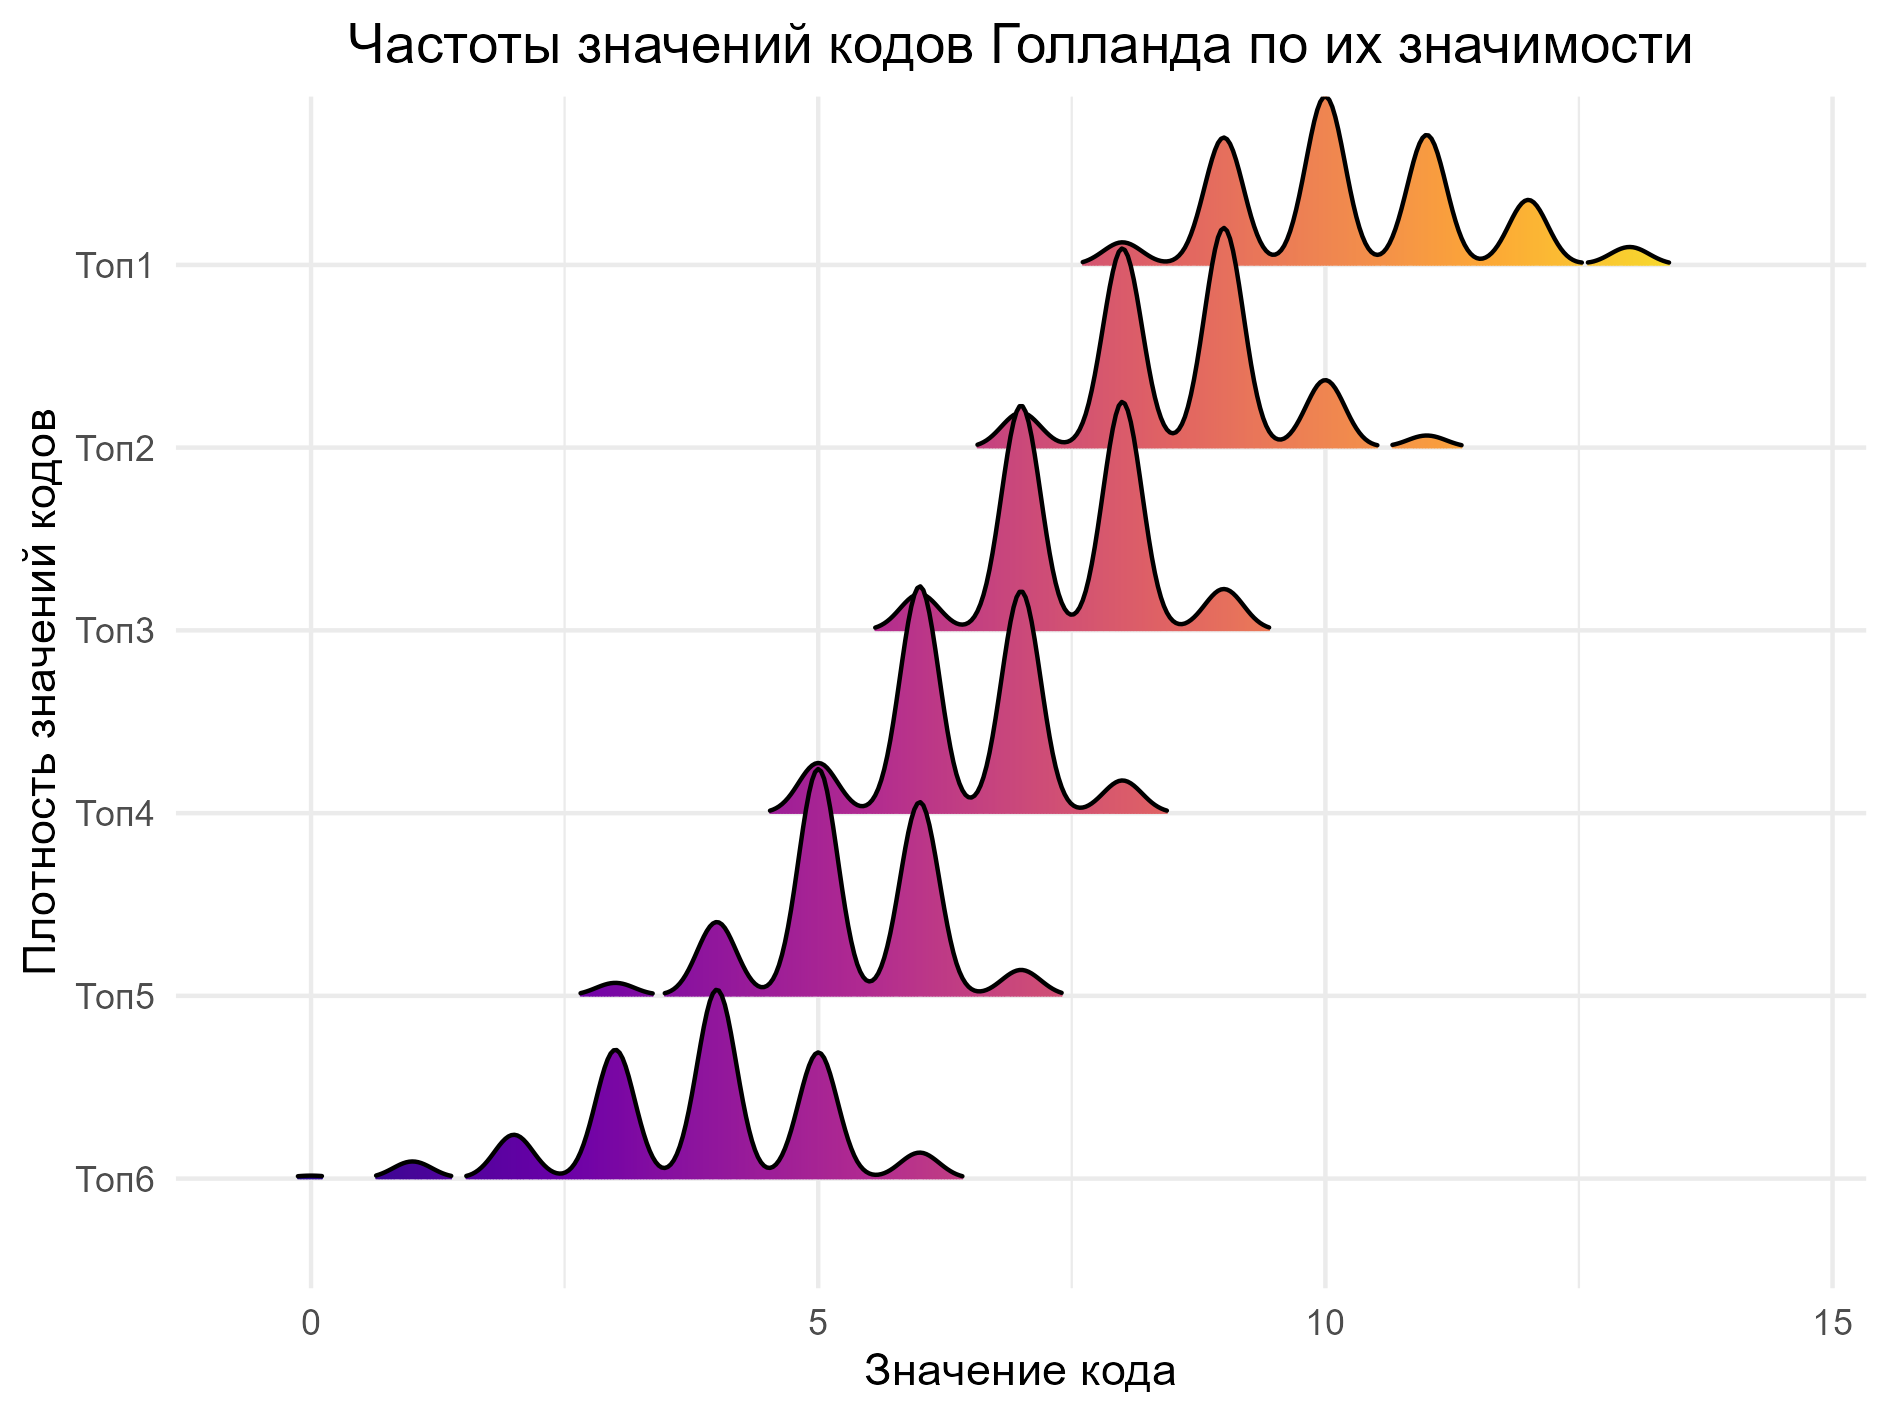
\includegraphics[width=\linewidth]{figures/ranks.png}
        \caption{Частоты значений кодов Голланда в порядке убывания их значимости}
        \label{fig:ranks}
    \end{minipage}
\end{figure}

Для анализа линейных связей между факторами модели Голланда на рисунке~\ref{fig:HL_cor} приведена матрица корреляций: коэффициент корреляции Пирсона по модулю не превышает $0.4$ (умереннная зависимость). Описательная статистика по всем факторам всех психометрических тестов приведена в Приложении~\ref{app:psytests} в таблице~\ref{tab:psytests_desc_stats}. Каждый из представленных факторов является числовой метрической переменной, принимающей только целочисленные значения.

\begin{figure}[bhtp]
    \centering
    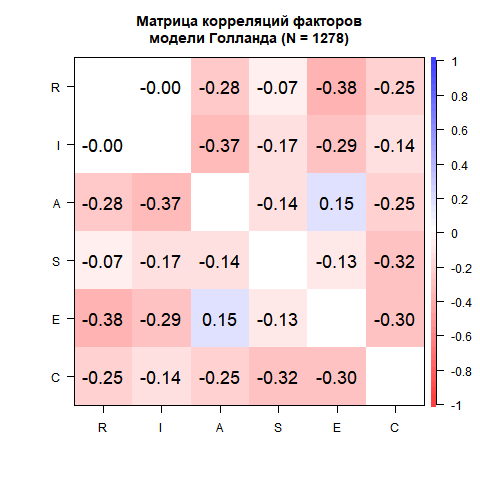
\includegraphics[width=0.6\linewidth]{figures/cor_united.png}
    \caption{Матрица корреляций кодов Голланда}
    \label{fig:HL_cor}
\end{figure}

К основным ограничениям исследования относятся особенности сбора данных: возможны смещения из-за специфики портала, а также способа формирования выборки. Для устранения ограничений может быть увеличен размер выборки, включены вопросы о социально-демографических признаках опрашиваемых.


\subsection{Особенности реализации модулей программного инструмента}

\subsubsection{Модуль обработки и восстановления данных}

Данные по пройденным пользователями тестам были получены в json-формате, где пользователю поставлен в соответствие пройденный им тест с результатами. Данные были преобразованы в \enquote{широкий} табличный формат, заполнены самоочевидные пропуски (исходя из природы психометрических данных), проведена валидация данных в соответствии с допустимыми значениями каждого из факторов психометрических тестов. Для проведения вычислительного эксперимента данные были поделены на обучающую, валидационную и тестовую выборки. Нормализация (стандартизация) данных всех выборок происходит в соответствии со средним значением и с значением стандартного отклонения, вычисляемым по обучающей выборке (функции \lstinline{transform_data_to_wide}, \lstinline{train_test_split} в программном коде).

Уменьшение размерности было реализовано в виде метода главных компонент (PCA) с помощью библиотеки \emph{stats}, функции \lstinline{prcomp}. В результате набора экспериментов было найдено, что чаще всего наилучший результат обеспечивает снижение размерности до 90\% объясняемой дисперсии, а именно до 30 компонент; таким образом, сравнение моделей велось и на полном наборе данных, и на данных меньшей размерности ($N_{comp} = 30$). В дальнейшем для моделей (если не указано иное) итоговое значение метрики~--- это лучшее из значений метрики модели на полном наборе данных и на наборе меньшей размерности.

Восстановление значений факторов незаполненных психометрических тестов для множественной импутации реализовано в функции \lstinline{mice_imputation} (в основе лежит реализация из библиотеки \emph{mice}); низко\-ранговая матричная аппрокси\-мация (\mbox{листинг}~\ref{lst:softimpute})~--- \lstinline{train_matrix_completion} для учета зависимостей и \lstinline{transform_matrix_completion} для преобразования с использованием библиотеки \emph{softImpute}; \lstinline{prepare_mask_data} для применения масок.

\begin{listing}
    \caption{Низкоранговая матричная аппроксимация \emph{Soft Impute}}
    \label{lst:softimpute}
    \begin{minted}[frame=lines]{r}
train_matrix_completion <- function(DT, rank.max = 20) {
  aux_feats <- setdiff(colnames(DT), c("id", paste0("HL_", 1:6)))
  M         <- as.matrix(DT)[, aux_feats]
  fit       <- softImpute::softImpute(M, rank.max = rank.max, lambda = 0, type = "als")
  return(list(fit = fit, aux = aux_feats))
}

transform_matrix_completion <- function(fit_obj, DT_new) {
  DT_new <- DT_new %>% as.matrix() %>%
    softImpute::complete(fit_obj$fit) %>%
    {DT_new[, fit_obj$aux] <- .; DT_new}
  return(DT_new)
}
  \end{minted}
\end{listing}


\subsubsection{Модуль обучения базовых моделей}

Базовые модели регрессии и классификации, перечисленные в подразделах~\ref{subsec:regr} и~\ref{subsec:classif}, в языке R реализованы в различных пакетах: линейная регрессия (\emph{lm}) в пакете \emph{stats}, регуляризованная регрессия~--- \emph{glmnet}, пошаговая~--- \emph{MASS}; одноимённые модели в пакетах \emph{xgboost}, \emph{lightgbm}, \emph{catboost}, \emph{randomForest}; метод k-ближайших соседей в \emph{FNN} и \emph{caret}; метод опорных векторов и наивный байесовский классификатор в \emph{e1071}; алгоритм ExtraTrees в \emph{ranger}. Для проведения экспериментов разработан унифицированный интерфейс взаимодействия с моделями: с помощью пакета \emph{R6} реализованы соответствующие классы-обёртки, наследующие шаблонный класс \lstinline{my_template_model}, в которых при необходимости переопределены методы \lstinline{initialize()}, \lstinline{fit()} и \lstinline{predict()}. Многие модели, например, случайный лес, бустинги, линейные регрессии, позволяют вычислять важность признаков, поэтому для них определен метод \lstinline{calc_importance()}.

Для решения задачи регрессии с помощью нейронных сетей был взят язык \emph{Python} и фреймворк \emph{PyTorch}. Первая модель из трёх реализованных представляет собой простой многослойный перцептрон с четырьмя плотными слоями ($55 \rightarrow 128 \rightarrow 64 \rightarrow 32 \rightarrow 6$) и функцией активации ReLU: такое снижение размерности позволяет постепенно выделять всё более абстрактные признаки из исходных 55 факторов и сразу выдавать шесть прогнозируемых значений. Вторая модель расширена модулями нормализации (BatchNorm) и регуляризации (Dropout, L1/L2-регуляризация, весовой спад) на каждом скрытом слое, что улучшает сходимость, устойчивость к переобучению и ускоряет обучение: сочетание таких приёмов и глубины должно обеспечивать баланс между выразительностью сети и её обобщающей способностью. В качестве третьей модели используется \emph{TabPFN} (библиотека \emph{tabpfn})~--- это трансформер, предобученный на большом числе синтетических табличных задач и предлагающий встроенную байесовскую оценку неопределённости. Он позволяет мгновенно делать предсказания без итеративного обучения, автоматически адаптируясь к различным типам признаков и небольшим объёмам данных. Модель \emph{TabPFN} также демонстрирует стабильные результаты в условиях разнородных и зашумлённых данных.

Решение задачи ранжирования также было реализовано в \emph{Python} с помощью \emph{PyTorch} (подклассы \lstinline{nn.Module}). Для списочного ранжирования были реализованы три класса:
\begin{itemize}
    \item \lstinline{MLPRanker} включает четыре полносвязных слоя размерности [$55 \rightarrow 128 \rightarrow 64 \rightarrow 32 \rightarrow 6$] с последовательным применением BatchNorm и Dropout. Такая глубина позволяет постепенно снижать размерность признаков и выделять всё более абстрактные комбинации без избыточного роста числа параметров.
    \item \lstinline{DCNUserItemRanker} сочетает три перекрёстных (\emph{cross}) слоя, моделирующих полиномиальные взаимодействия входных признаков, и \enquote{глубокую} ветвь из линейных блоков [$64 \rightarrow 128 \rightarrow 64 \rightarrow 32$] с ReLU и Dropout. Число перекрёстных слоёв выбрано эмпирически: трёх итераций перекрёстных преобразований достаточно для учёта основных взаимодействий, при этом обучение остаётся устойчивым.
    \item Модель \lstinline{ListwiseTransformer} для каждого из шести элементов создаёт обучаемое представление (эмбеддинг) размерности 8, объединяет его с 55-мерным входным вектором, затем проецирует результат в пространство размерности 64 (\lstinline{d_model = 64}). Далее он проходит через два слоя кодировщика на основе трансформера с четырьмя головами внимания (\lstinline{nhead = 4}) и завершается одним линейным выходным слоем. Использование двух слоёв обеспечивает баланс между учётом взаимного влияния элементов и приемлемым временем обучения.
\end{itemize}
Каждый из классов комбинируется с четырьмя функциями ошибок, соответствующих списочной оптимизации:
\begin{itemize}
    \item \lstinline{ListNet@1} и \lstinline{ListNet@3} вычисляют кросс-энтропию между распределениями рангов (полным или усечённым до топ-3) с помощью функции \lstinline{softmax};
    \item \lstinline{ApproxNDCG} аппроксимирует классическую метрику NDCG, вводя дифференцируемые ранги через сигмоидные функции;
    \item \lstinline{LambdaRank} формирует парно-ориентированную функцию ошибок с расчётом $\lambda$-коэффициентов на основе $\Delta\mathrm{NDCG}$ при перестановках.
\end{itemize}

\begin{listing}
    \caption{Функция подсчета важности моделей на основе вектора Шэпли (с применением стохастического метода Монте-Карло)}
    \label{lst:weight_optim_shap}
    \begin{minted}[frame=lines]{r}
approx_shapley <- function(models_probs, Y_true, R = 500) {
  M <- length(models_probs)
  prob_array <- simplify2array(models_probs)
  phi <- numeric(M)
  for (r in seq_len(R)) {
    perm <- sample.int(M)
    cum_sum <- 0
    v_prev <- 0
    for (k in seq_along(perm)) {
      idx <- perm[k]
      cum_sum <- cum_sum + prob_array[,, idx]
      v_curr <- matr_cind(cum_sum / k, Y_true)
      phi[idx] <- phi[idx] + (v_curr - v_prev)
      v_prev <- v_curr
    }
  }
  w <- phi / R
  return(w / sum(w))
}
  \end{minted}
\end{listing}


\subsubsection{Модуль формирования взвешенного ансамбля моделей}

Подбор весов моделей для дальнейшего взвешенного ансамблирования (линейного блендинга) был реализован в следующих функциях:
\begin{itemize}
    \item равные веса всех моделей~--- функция \lstinline{equal_weights};
    \item вектор Шэпли~--- \lstinline{approx_shapley} (листинг~\ref{lst:weight_optim_shap}). Для ускорения работы функции производилась стохастическая аппроксимация с использованием метода Монте-Карло: вместо полного перебора всех вариантов были выбраны \emph{R} перестановок (разброс значений оценок уменьшается пропорционально $1/\sqrt{R}$);
    \item частичный перебор по сетке~--- \lstinline{grid_search_weights} с заданием шага сетки;
    \item квадратичная оптимизация в функции \lstinline{stacking_qp_weights}, использующая функцию \lstinline{solve.QP} библиотеки \emph{quadprog};
    \item генетический алгоритм и метод роя частиц~--- реализованы на основе функций \lstinline{ga} библиотеки \emph{GA} и \lstinline{psoptim} из \emph{PSO} (код функции \lstinline{particle_swarm_weights} приведен в листинге~\ref{lst:weight_optim_pso});
    \item координатный спуск~--- функция \lstinline{coordinate_optimize_weights} (использует библиотеку \emph{stats}).
\end{itemize}

От использования подбора весов с помощью байесовской оптимизации (библиотека \emph{rBayesianOptimization}) было решено отказаться вследствие больших вычислительных затрат (разница во времени выполнения, например, с методом роя частиц в два порядка).

Таким образом, способы подбора весов были реализованы как собственными средствами, так и с использованием возможностей, встроенных в различные пакеты.

\begin{listing}
    \caption{Функция подсчета важности моделей на основе метода роя частиц (PSO)}
    \label{lst:weight_optim_pso}
    \begin{minted}[frame=lines]{r}
particle_swarm_weights <- function(models_probs, Y_true, swarm_size = 50, maxit = 100) {
  M <- length(models_probs)
  fn_pso <- function(x) {-weighted_cindex_value(x / sum(x), models_probs, Y_true)}
  PSOres <- pso::psoptim(par = rep(1/M, M), fn = fn_pso, lower = rep(.Machine$double.eps, M), upper = rep(1, M), control = list(s = swarm_size, maxit = maxit, trace = FALSE, vectorize = TRUE, maxit.stagnate = 10))
  w <- PSOres$par
  w[w < 1e-6] <- 0
  return(w / sum(w))
}
  \end{minted}
\end{listing}


\subsubsection{Модуль организации и проведения вычислительных экспериментов}

При разработке решения задачи многоцелевой регрессии были реализованы походы независимого предсказания выходов (значений кодов Голланда) \lstinline{stack_MO_regr}, предсказаний по цепочке \lstinline{chain_MO_regr} и \lstinline{no_MO_regr} для предсказаний моделей, поддерживающих множественные выходы по умолчанию. Наличие унифицированных интерфейсов (R6-классов) с базовыми моделями позволило организовать массовую оценку моделей с помощью функции \lstinline{calc_regression_models}, на вход которой подается следующий набор данных: название класса модели, её метка и гиперпараметры, подход к многоцелевой регрессии; код представлен в листинге~\ref{lst:calc_regr}. Аналогичный подход был использован для реализации подходов к решению задачи классификации: на основе унифицированной функции-интерфейса \lstinline{classification_test_framework}, позволяющего обучить модель, сделать предсказание, оценить значения метрик качества (C-индекс и точность Top-K), применяется функция, например, \lstinline{run_multilabel_experiments} для многометочной классификации (листинг~\ref{lst:multilabel_clsf}).

\begin{listing}
    \caption{Функция массовой оценки регрессионных моделей}
    \label{lst:calc_regr}
    \begin{minted}[frame=lines]{r}
calc_regression_models <- function(regr_models_df, X_train_, Y_train_, X_test_, Y_test_) {
  MO_res <- regr_models_df %>% 
    copy() %>% 
    .[, pred := pmap(list(model, params, MO_type), \(mdl, par, mo_type) do.call(perform_MO_regression, 
        c(list(mdl, mo_type, X_train_, Y_train_, X_test_, Y_test_, print_model_name = F), par)))] %>% 
    .[, rmse := map_dbl(pred, \(x) df_metric(x, Y_test_, my_rmse) %>% round(3))] %>% 
    .[map_lgl(pred, \(item) !is.null(item)),
      C_index := map_dbl(pred, \(x) df_metric(x, Y_test_, calc_C_index) %>% round(3))] %>% 
    .[, .(name, pred, rmse, C_index)]
  return(MO_res)
}
  \end{minted}
\end{listing}

\begin{listing}
    \caption{Функция массовой оценки решения задачи многометочной классификации}
    \label{lst:multilabel_clsf}
    \begin{minted}[frame=lines]{r}
run_multilabel_experiments <- function(experiments_df, X_train, Y_b_train, 
                                       X_test, Y_b_test) {
  # experiments_df (tibble/data.table): clsf_func, label, params, n_retry
  evaluate_ML <- function(multlbl_clsf_func, label = "", n_retry = 1, ...) {
    classification_test_framework(Y_test = Y_b_test, Y_b_test = Y_b_test, 
                                  clsf_func = multlbl_clsf_func, n_retry = n_retry, 
                                  label = label, X_train = X_train, 
                                  Y_b_train = Y_b_train, X_test = X_test, ...)
  }
  
  res <- experiments_df %>%
    as.data.table() %>%
    .[, metrics := pmap(list(multlbl_clsf_func, label, params, n_retry), \(ind_fn, lbl, extra_args, nr) 
                        do.call(evaluate_ML, c(list(multlbl_clsf_func = ind_fn, label = lbl, n_retry = nr), extra_args))
    )] %>%
    .[, .(label, metrics, id = 1:.N)] %>%
    .[, metrics[[1]], by = id]
  
  return(res)
}
  \end{minted}
\end{listing}


\subsection{Реализация прототипа инструмента для определения профориентационных предпочтений}

Прототип инструмента для определения профориентационных предпочтений был реализован в виде интерактивного веб-приложения на платформе R Shiny. На рисунке~\ref{fig:pipeline} приведён общий порядок вычислительного конвейера разработанного прототипа программного инструмента, в котором последовательно выполняются все необходимые шаги: от предобработки и очистки исходных данных до восстановления пропусков с помощью модели мягкого матричного восстановления \emph{Soft Impute} и дальнейшего прогнозирования с помощью предварительно обученной и сохраненной модели регуляризованной L1-регрессии (\emph{Lasso}), показавшей наилучшие результаты среди базовых моделей (при оценке C-индекса).

\begin{figure}[htbp]
    \centering
    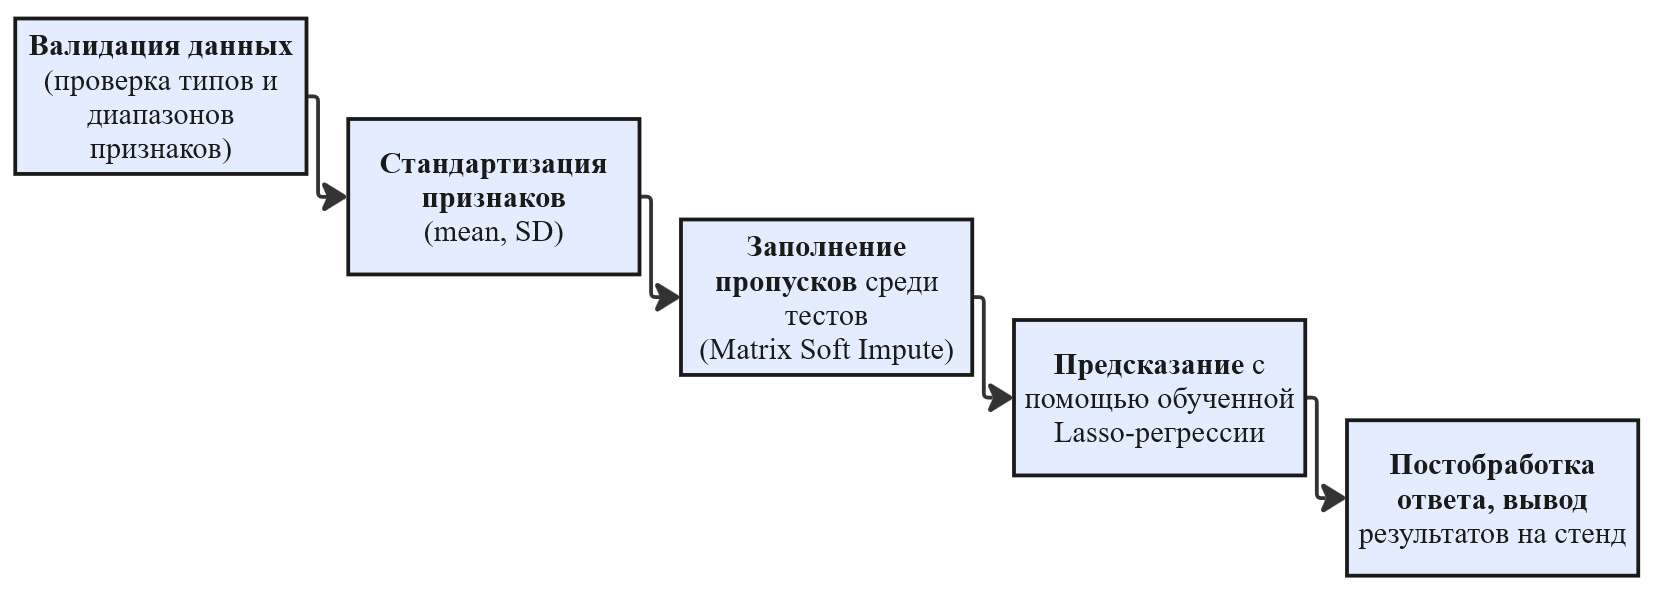
\includegraphics[width=1.0\linewidth]{figures/final_pipeline.jpg}
    \caption{Итоговая последовательность вычислительных шагов}
    \label{fig:pipeline}
\end{figure}

При разработке веб-стенда на R Shiny в блоке кода \lstinline{ui} через \lstinline{fluidPage} и \lstinline{bsCollapse} с помощью функции \lstinline{create_test_ui} динамически формируется панель тестов с групповыми сворачивающимися блоками вопросов. В серверной части с помощью \lstinline{reactiveValues} для хранения промежуточных данных и \texttt{observeEvent(input\$calc)} организована реактивная логика: при нажатии \enquote{Подсчитать} происходит валидация входных значений (в случае выхода за рамки допустимых значений пользователю выводится сообщение об ошибке), восстановление пропусков методом \emph{Soft Impute} и нормализация данных, затем вызывается функция предсказания, а результаты выводятся через \lstinline{renderUI} и подтверждаются уведомлениями \lstinline{showNotification}. По завершении вычислений результаты в виде набора кодов рекомендуемых направлений сопровождаются подробным текстовым описанием и визуальной презентацией на пользовательском интерфейсе (см. интерфейс стенда на рисунках~\ref{fig:ui} и~\ref{fig:ui2}). Разделение на \lstinline{ui} и \lstinline{server} типично для \emph{Shiny}-приложений: \lstinline{ui} описывает компоненты интерфейса, а сервер~--- реактивную логику и обновление данных. Такой подход обеспечивает раздельную ответственность за внешний вид и вычислительную логику прототипа.

Доступ к приложению не требует процедуры авторизации, при этом его развертывание возможно как в локальной среде, так и на удалённом сервере с использованием средств хостинга. Разработанный прототип может быть использован в составе более комплексных информационных систем, направленных на поддержку профессиональной ориентации и образовательного планирования.

\begin{figure}[htbp]
    \centering
    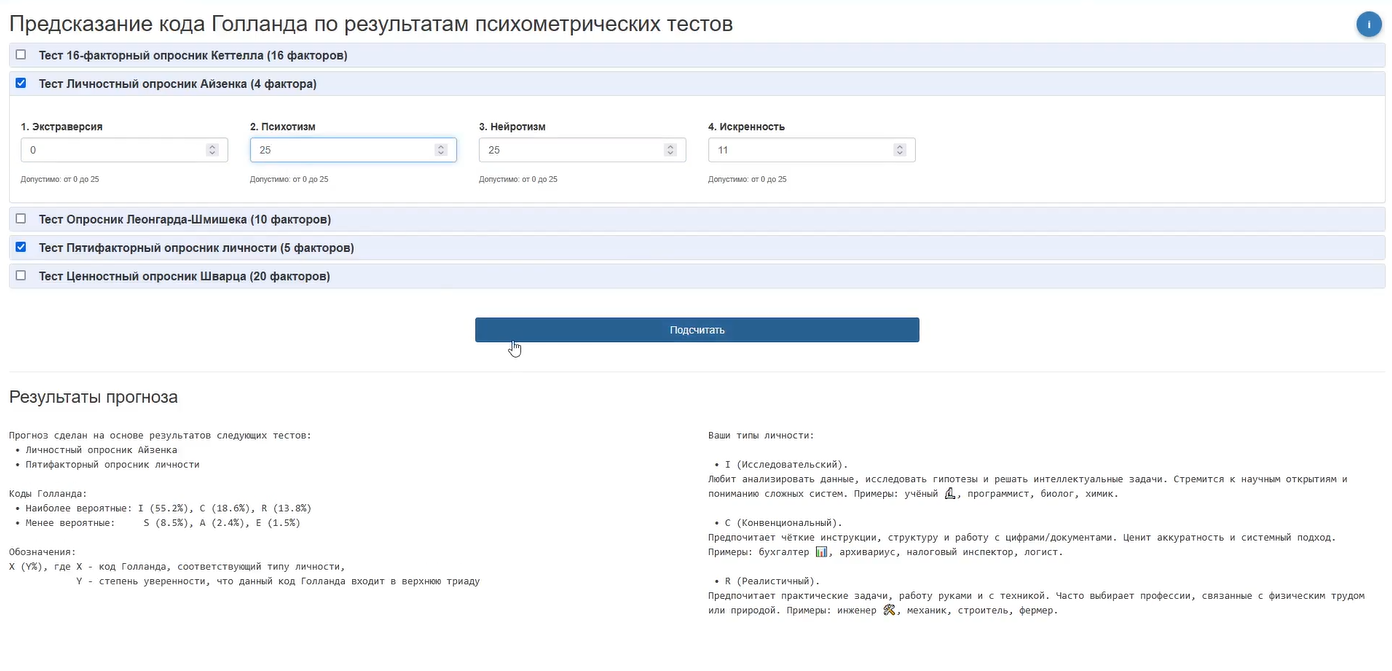
\includegraphics[width=1.0\linewidth]{figures/UI1.png}
    \caption{Интерфейс прототипа инструмента профориентации}
    \label{fig:ui}
\end{figure}
